\chapter{Vergleich der Ergebnisse}




%Kohärenz, Distanz, Themenanzahl, Verständlichkeit, Aufwand
\section{Kennzahlen}

Die Unigrammmodelle weisen eine niedrigere Distanz zueinander auf als die Bigrammmodelle. In Abbildung 4.1 sind schon Muster und Hotspots aus Unigrammthemen zu erkennen, die besonders Ähnlich oder unähnlich sind. Diese werden später geclustered. In Abbildung 4.2 gibt es ebenfalls Muster und Hotspots. Allerdings sind manche Bigrammthemen disjunkt.

\begin{figure}[htpb]
	\centering
	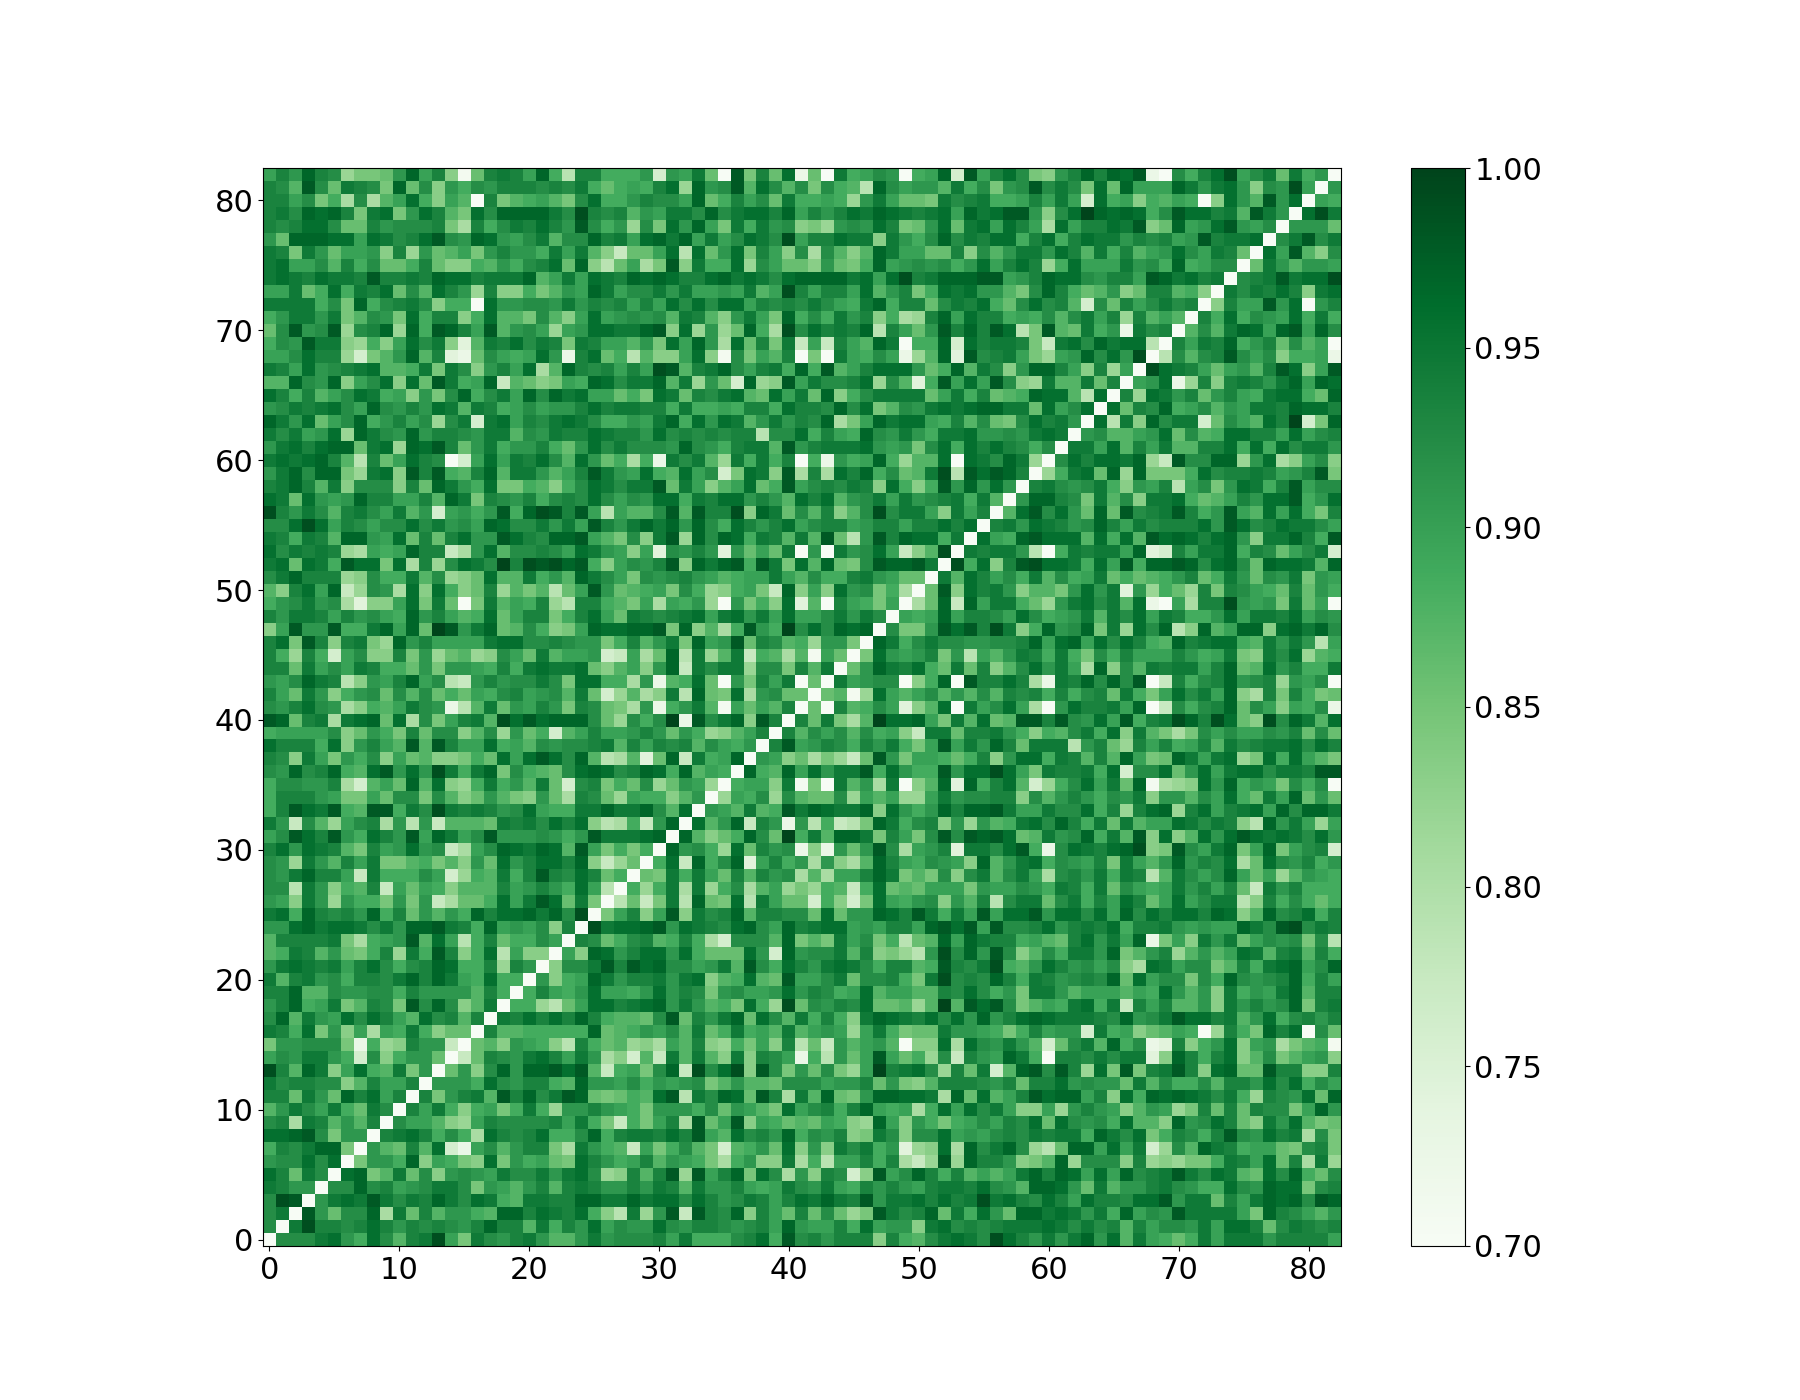
\includegraphics[width=\textwidth,height=12cm,keepaspectratio=true]{img/unigram_jaccard_50_green_07.png}
	\caption{
		Distanz zwischen den top 50 Unigrammen der Themen
	}
	\label{fig:Distanz_Unigramme}
\end{figure}

\begin{figure}[htpb]
	\centering
	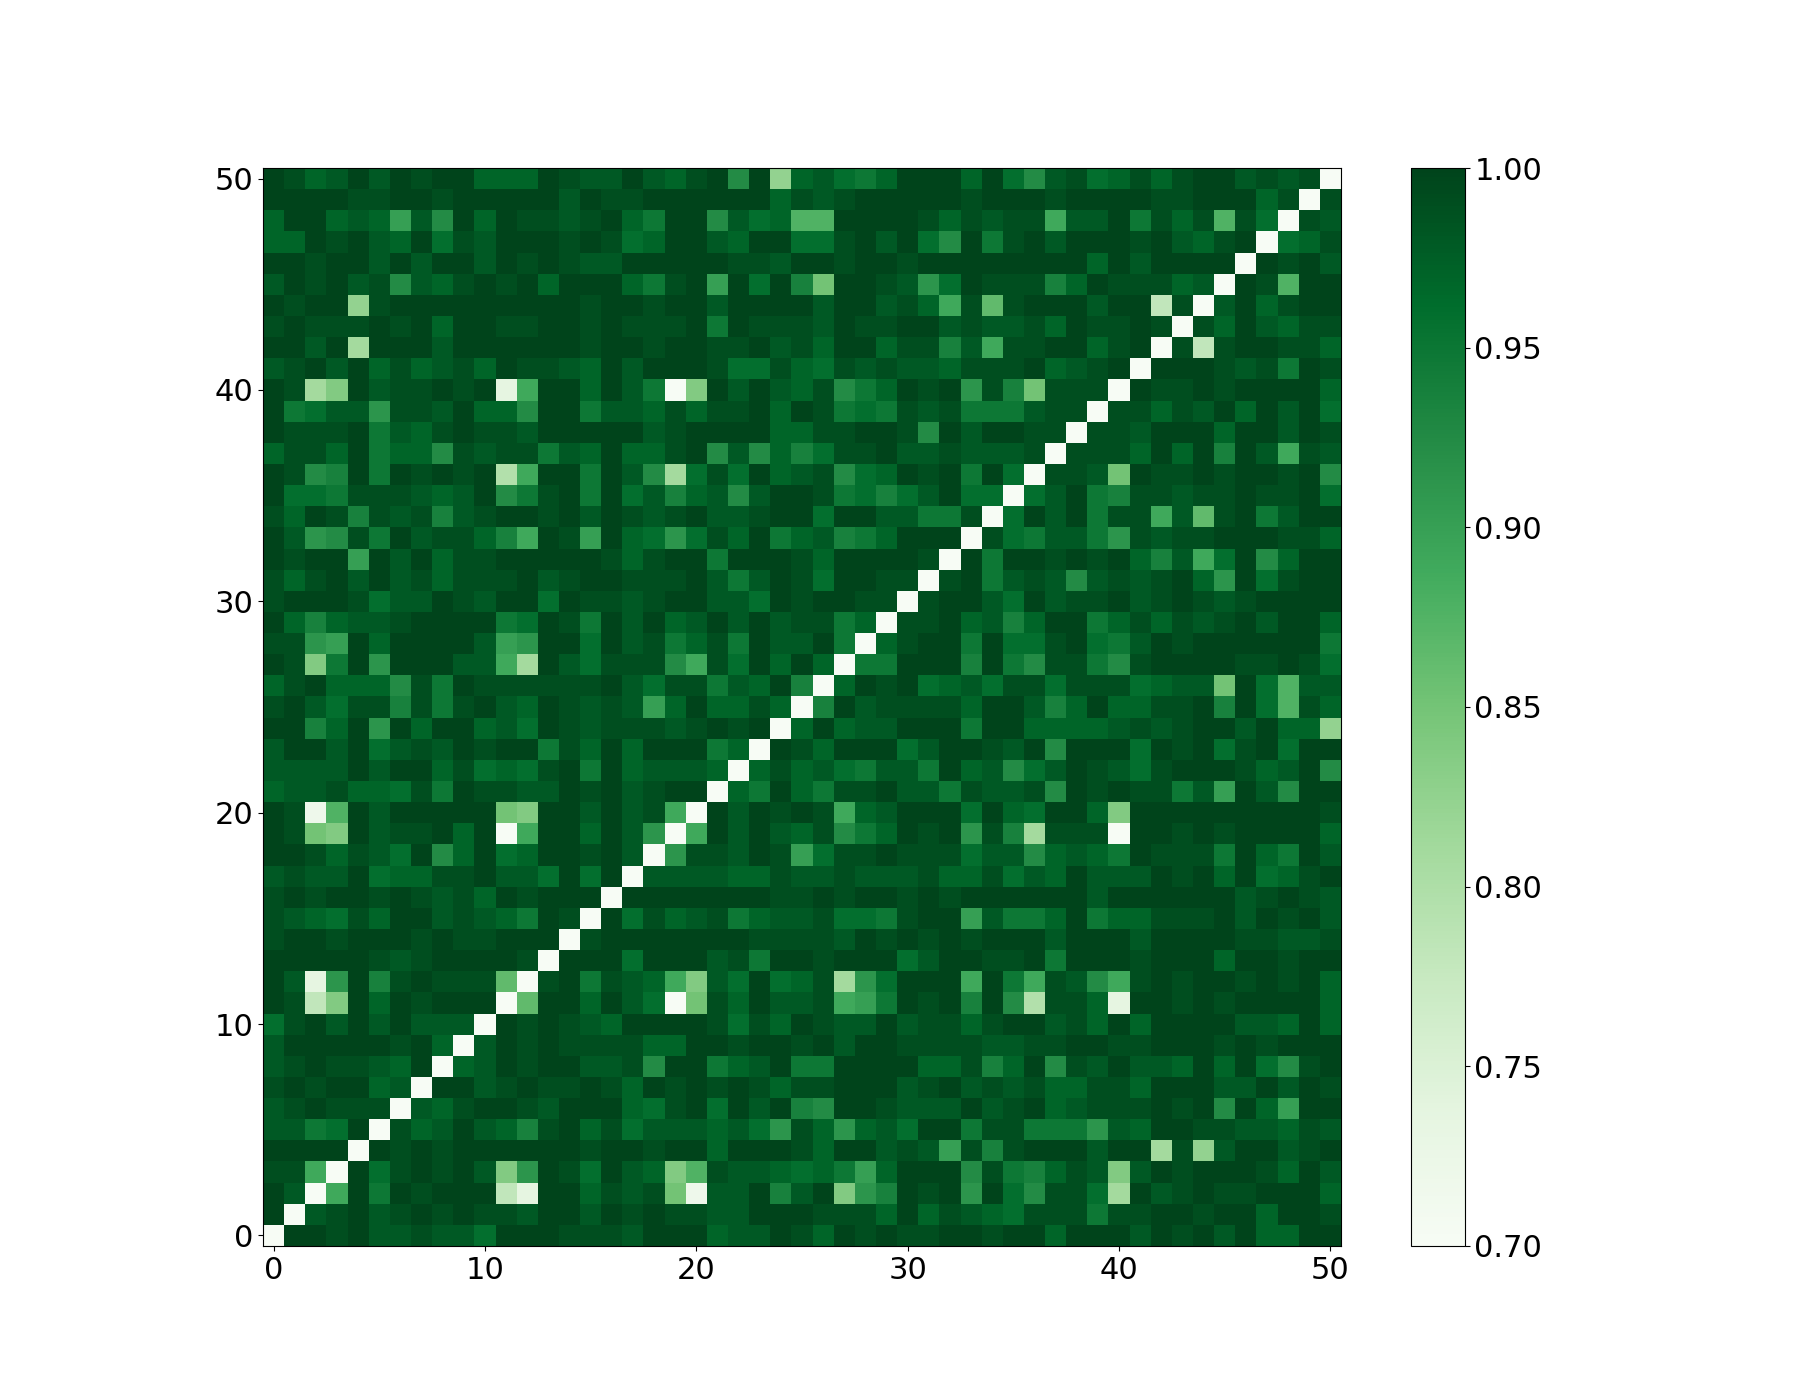
\includegraphics[width=\textwidth,height=12cm,keepaspectratio=true]{img/bigram_jaccard_50_green_07.png}
	\caption{
		Distanz zwischen den top 50 Bigrammen der Themen
	}
	\label{fig:Distanz_Bigramme}
\end{figure}


\section{Themengruppen}

LDA

\begin{figure}[htpb]
	\centering
	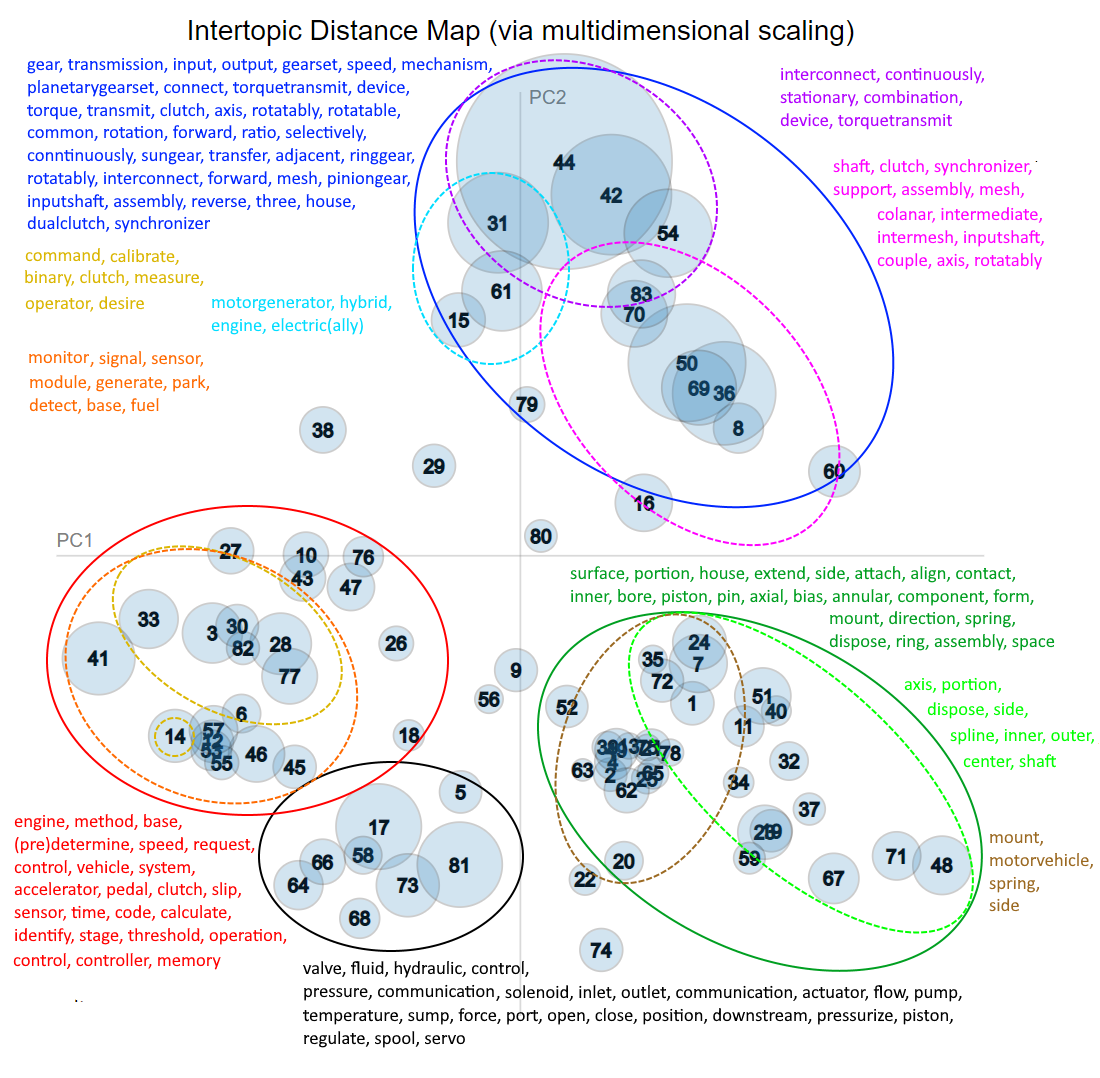
\includegraphics[width=\textwidth,height=10cm,keepaspectratio=true]{img/LDAvisGM-3-1-1clustered.png}
	\caption{
		Themengruppen der LDA Unigramme
	}
	\label{fig:Themengruppen_LDA_Unigramm}
\end{figure}


DLDA

HLDA

\section{Interpretation der Themen}

LDA

DLDA

HLDA
